% Options for packages loaded elsewhere
\PassOptionsToPackage{unicode}{hyperref}
\PassOptionsToPackage{hyphens}{url}
\PassOptionsToPackage{dvipsnames,svgnames,x11names}{xcolor}
%
\documentclass[
  12pt]{article}

\usepackage{amsmath,amssymb}
\usepackage{iftex}
\ifPDFTeX
  \usepackage[T1]{fontenc}
  \usepackage[utf8]{inputenc}
  \usepackage{textcomp} % provide euro and other symbols
\else % if luatex or xetex
  \usepackage{unicode-math}
  \defaultfontfeatures{Scale=MatchLowercase}
  \defaultfontfeatures[\rmfamily]{Ligatures=TeX,Scale=1}
\fi
\usepackage{lmodern}
\ifPDFTeX\else  
    % xetex/luatex font selection
\fi
% Use upquote if available, for straight quotes in verbatim environments
\IfFileExists{upquote.sty}{\usepackage{upquote}}{}
\IfFileExists{microtype.sty}{% use microtype if available
  \usepackage[]{microtype}
  \UseMicrotypeSet[protrusion]{basicmath} % disable protrusion for tt fonts
}{}
\makeatletter
\@ifundefined{KOMAClassName}{% if non-KOMA class
  \IfFileExists{parskip.sty}{%
    \usepackage{parskip}
  }{% else
    \setlength{\parindent}{0pt}
    \setlength{\parskip}{6pt plus 2pt minus 1pt}}
}{% if KOMA class
  \KOMAoptions{parskip=half}}
\makeatother
\usepackage{xcolor}
\setlength{\emergencystretch}{3em} % prevent overfull lines
\setcounter{secnumdepth}{5}
% Make \paragraph and \subparagraph free-standing
\makeatletter
\ifx\paragraph\undefined\else
  \let\oldparagraph\paragraph
  \renewcommand{\paragraph}{
    \@ifstar
      \xxxParagraphStar
      \xxxParagraphNoStar
  }
  \newcommand{\xxxParagraphStar}[1]{\oldparagraph*{#1}\mbox{}}
  \newcommand{\xxxParagraphNoStar}[1]{\oldparagraph{#1}\mbox{}}
\fi
\ifx\subparagraph\undefined\else
  \let\oldsubparagraph\subparagraph
  \renewcommand{\subparagraph}{
    \@ifstar
      \xxxSubParagraphStar
      \xxxSubParagraphNoStar
  }
  \newcommand{\xxxSubParagraphStar}[1]{\oldsubparagraph*{#1}\mbox{}}
  \newcommand{\xxxSubParagraphNoStar}[1]{\oldsubparagraph{#1}\mbox{}}
\fi
\makeatother


\providecommand{\tightlist}{%
  \setlength{\itemsep}{0pt}\setlength{\parskip}{0pt}}\usepackage{longtable,booktabs,array}
\usepackage{calc} % for calculating minipage widths
% Correct order of tables after \paragraph or \subparagraph
\usepackage{etoolbox}
\makeatletter
\patchcmd\longtable{\par}{\if@noskipsec\mbox{}\fi\par}{}{}
\makeatother
% Allow footnotes in longtable head/foot
\IfFileExists{footnotehyper.sty}{\usepackage{footnotehyper}}{\usepackage{footnote}}
\makesavenoteenv{longtable}
\usepackage{graphicx}
\makeatletter
\def\maxwidth{\ifdim\Gin@nat@width>\linewidth\linewidth\else\Gin@nat@width\fi}
\def\maxheight{\ifdim\Gin@nat@height>\textheight\textheight\else\Gin@nat@height\fi}
\makeatother
% Scale images if necessary, so that they will not overflow the page
% margins by default, and it is still possible to overwrite the defaults
% using explicit options in \includegraphics[width, height, ...]{}
\setkeys{Gin}{width=\maxwidth,height=\maxheight,keepaspectratio}
% Set default figure placement to htbp
\makeatletter
\def\fps@figure{htbp}
\makeatother

\addtolength{\oddsidemargin}{-.5in}%
\addtolength{\evensidemargin}{-1in}%
\addtolength{\textwidth}{1in}%
\addtolength{\textheight}{1.7in}%
\addtolength{\topmargin}{-1in}%
\makeatletter
\@ifpackageloaded{caption}{}{\usepackage{caption}}
\AtBeginDocument{%
\ifdefined\contentsname
  \renewcommand*\contentsname{Table of contents}
\else
  \newcommand\contentsname{Table of contents}
\fi
\ifdefined\listfigurename
  \renewcommand*\listfigurename{List of Figures}
\else
  \newcommand\listfigurename{List of Figures}
\fi
\ifdefined\listtablename
  \renewcommand*\listtablename{List of Tables}
\else
  \newcommand\listtablename{List of Tables}
\fi
\ifdefined\figurename
  \renewcommand*\figurename{Figure}
\else
  \newcommand\figurename{Figure}
\fi
\ifdefined\tablename
  \renewcommand*\tablename{Table}
\else
  \newcommand\tablename{Table}
\fi
}
\@ifpackageloaded{float}{}{\usepackage{float}}
\floatstyle{ruled}
\@ifundefined{c@chapter}{\newfloat{codelisting}{h}{lop}}{\newfloat{codelisting}{h}{lop}[chapter]}
\floatname{codelisting}{Listing}
\newcommand*\listoflistings{\listof{codelisting}{List of Listings}}
\makeatother
\makeatletter
\makeatother
\makeatletter
\@ifpackageloaded{caption}{}{\usepackage{caption}}
\@ifpackageloaded{subcaption}{}{\usepackage{subcaption}}
\makeatother
\ifLuaTeX
  \usepackage{selnolig}  % disable illegal ligatures
\fi
\usepackage[]{natbib}
\bibliographystyle{agsm}
\usepackage{bookmark}

\IfFileExists{xurl.sty}{\usepackage{xurl}}{} % add URL line breaks if available
\urlstyle{same} % disable monospaced font for URLs
\hypersetup{
  pdftitle={Apoorv Gupta and Jonathan Zinman: Coding Task},
  pdfauthor={William Co},
  colorlinks=true,
  linkcolor={blue},
  filecolor={Maroon},
  citecolor={Blue},
  urlcolor={Blue},
  pdfcreator={LaTeX via pandoc}}


\begin{document}


\def\spacingset#1{\renewcommand{\baselinestretch}%
{#1}\small\normalsize} \spacingset{1}


%%%%%%%%%%%%%%%%%%%%%%%%%%%%%%%%%%%%%%%%%%%%%%%%%%%%%%%%%%%%%%%%%%%%%%%%%%%%%%

\date{January 15, 2025}
\title{\bf Apoorv Gupta and Jonathan Zinman: Coding Task}
\author{
William Co\thanks{Thank you for the opportunity to complete this data
task for my predoctoral application. I appreciate your consideration,
and I look forward to meeting and contributing.}\\
Department of Economics, University of British Columbia\\
}
\maketitle

\bigskip
\bigskip
\begin{abstract}
This is a data task submitted for a predoctoral application, in
accordance with the guidelines outlined in the following document
https://github.com/WilliamClintC/Coding-Task-GuZi/blob/main/GZ\_RA\_StataTaskDescription.pdf
.
\end{abstract}


\newpage
\spacingset{1.9} % DON'T change the spacing!

\section{Introduction}\label{introduction}

I will be using quarto to construct this document per instruction
\citep{coCodingTaskGuZiGZ_RA_StataTaskDescriptionpdfMain2025}

The code for task 2 can be found here.
\href{https://github.com/WilliamClintC/Coding-Task-GuZi/tree/main/lottery_study/code}{link}
\citep{coCodingTaskGuZiLottery_studyCode2025}

\section{Task 1: Red Sox Ticket
Prices}\label{task-1-red-sox-ticket-prices}

\emph{How do the prices consumers pay for tickets change as the game
date approaches (i.e., as the number of days between transaction date
and game date declines)? How does this dynamic pattern change across
years?}

To address the question, we begin by running a preliminary regression to
gain a better understanding of our data. This regression includes all
available control variables and accounts for the number of tickets
purchased. Considering the potential for bulk discounts associated with
purchasing multiple tickets, we aim to capture variations in pricing
that may occur in different contexts, where such discounts might or
might not be offered.

\begin{enumerate}
\def\labelenumi{\arabic{enumi}.}
\item
  \textbf{Model with \texttt{number\_of\_tickets}}: \[
  \text{price\_per\_ticket} = \beta_0 + \beta_1 \cdot \text{days\_until\_game} + \beta_2 \cdot \mathbf{\text{controls}}  
  + \beta_3 \cdot \text{num\_tickets} + \epsilon
  \]
\item
  \textbf{Model without \texttt{number\_of\_tickets}}: \[
  \text{price\_per\_ticket} = \beta_0 + \beta_1 \cdot \text{days\_until\_game} + \beta_2 \cdot \mathbf{\text{controls}} + \epsilon
  \]
\item
  \textbf{Model with \texttt{number\_of\_tickets} using log price}: \[
  \log(\text{price\_per\_ticket}) = \beta_0 + \beta_1 \cdot \text{days\_until\_game} + \beta_2 \cdot \mathbf{\text{controls}} + 
  \beta_3 \cdot \text{num\_tickets} + \epsilon
  \]
\item
  \textbf{Model without \texttt{number\_of\_tickets} using log price}:
  \[
  \log(\text{price\_per\_ticket}) = \beta_0 + \beta_1 \cdot \text{days\_until\_game} + \beta_2 \cdot \mathbf{\text{controls}} + \epsilon
  \]
\end{enumerate}

Where: \[
\mathbf{\text{controls}} = \text{day\_game, weekend\_game, sectiontype, gamemonth, team, year}
\]

\begin{itemize}
\tightlist
\item
  \(\beta_0\) is the intercept.
\item
  \(\beta_1, \beta_3\) are the coefficients for the respective predictor
  variables.
\item
  \(\beta_2\) is a vector of coefficients for control variables.
\item
  \(\epsilon\) is the error term.
\end{itemize}

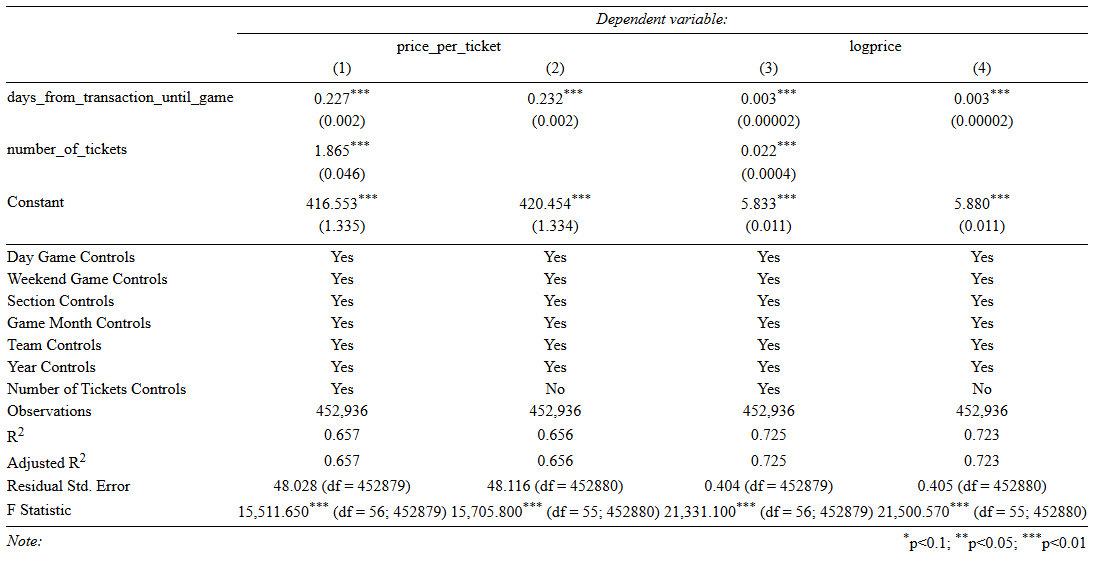
\includegraphics{images/0.png}

The results indicate that the earlier tickets are purchased, the more
expensive they tend to be, as evidenced by the positive and significant
coefficient on the variable
\texttt{days\_from\_transaction\_until\_game}. This finding is counter
intuitive. Typically, purchasing tickets earlier is expected to be less
expensive because it reduces the risk for the ticket vendor, smooths out
their cash flow, and provides an early cash injection. Additionally, the
time value of money suggests that receiving payments earlier should
incentivise lower prices.

To explore this unexpected result further, we conduct an investigation
using scatter plots.

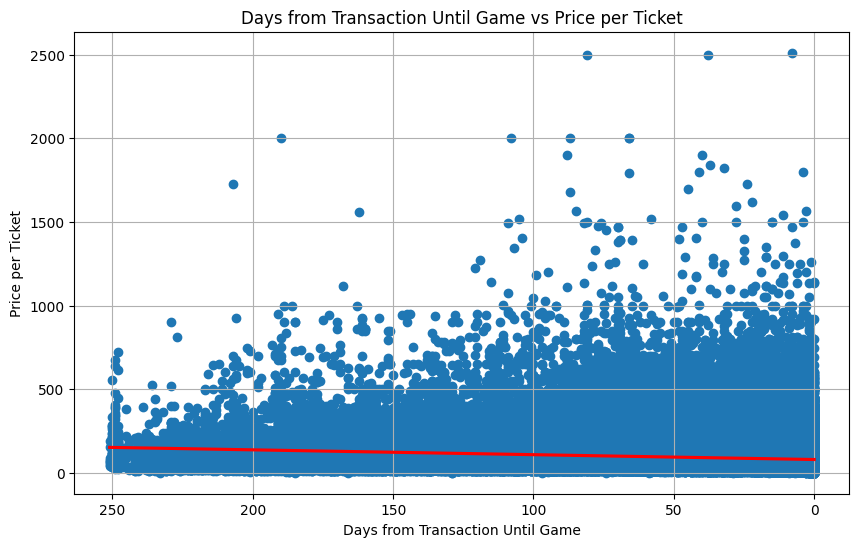
\includegraphics{images/16.png}

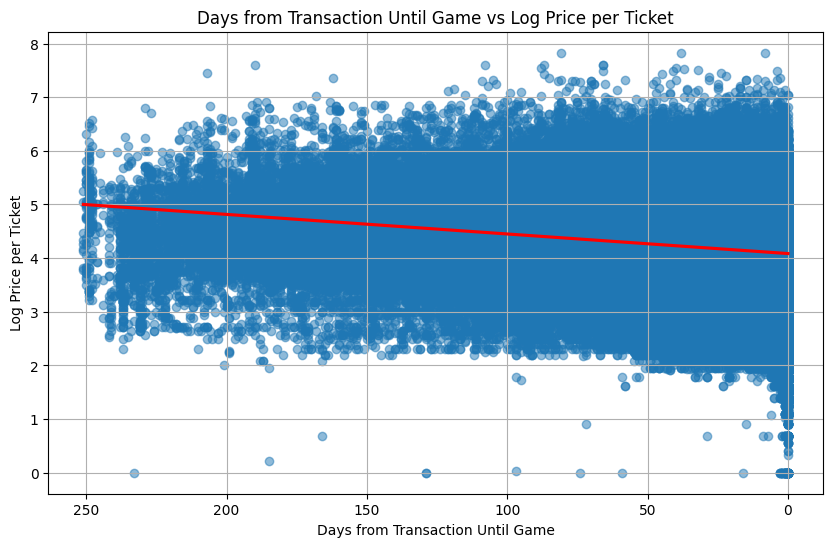
\includegraphics{images/17.png}

The relationship may be biased by noise. So this would warrant further
investigation. To investigate further, I look into the team with the
most observations (NYY). I also control for other attributes with the
most observation within NYY (LowerBleachers, 2 Tickets, April, Evening
and Weekend games in 2011). The following are my
results.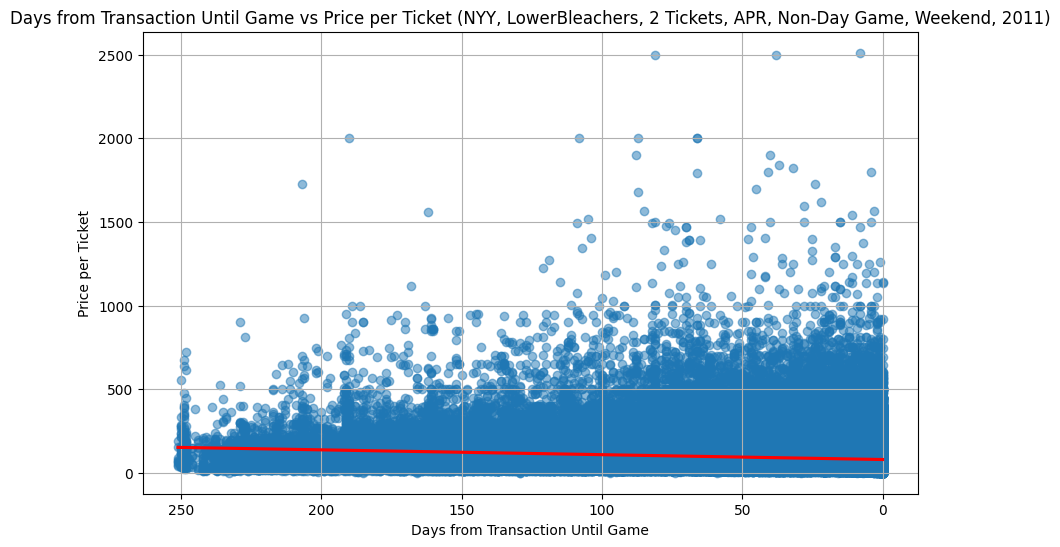
\includegraphics{images/18.png}

The results show similarity to the initial plots we observed from
earlier. I suspect the results from the data are due to some noise
introduced by price outliers. I clean the data of price outliers
manually and rerun the same regressions, mentioned prior.

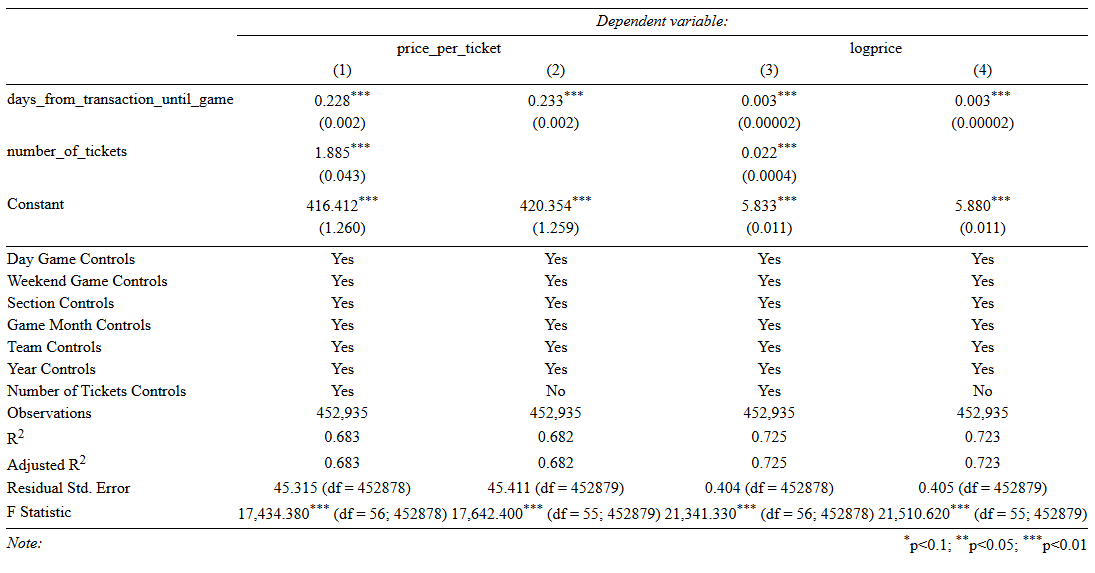
\includegraphics{images/5.png}

There does not seem to be any significant effect on the results. To
further investigate, we use bin scatter plots and show our results
again.

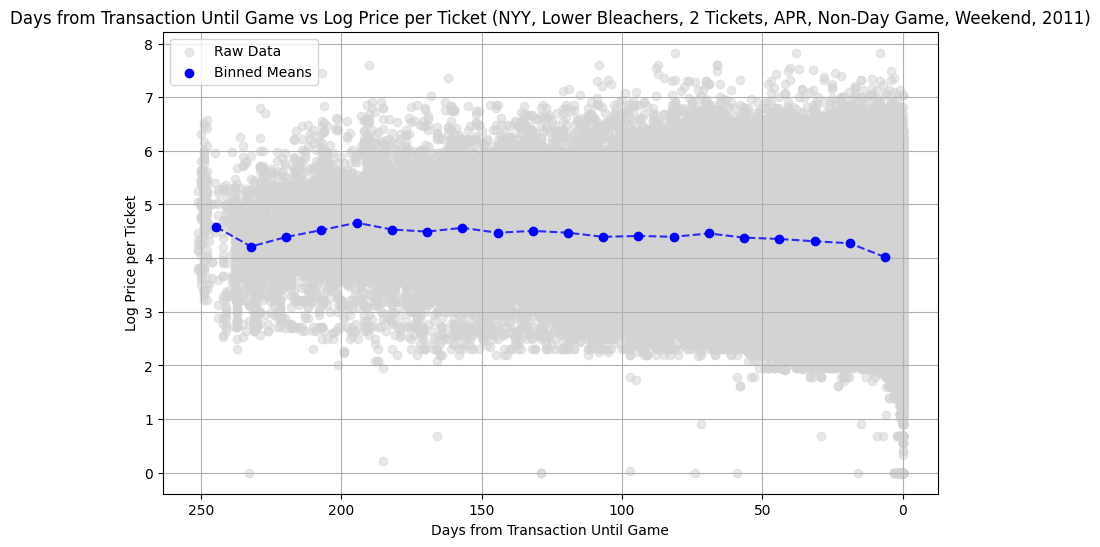
\includegraphics{images/11.png}

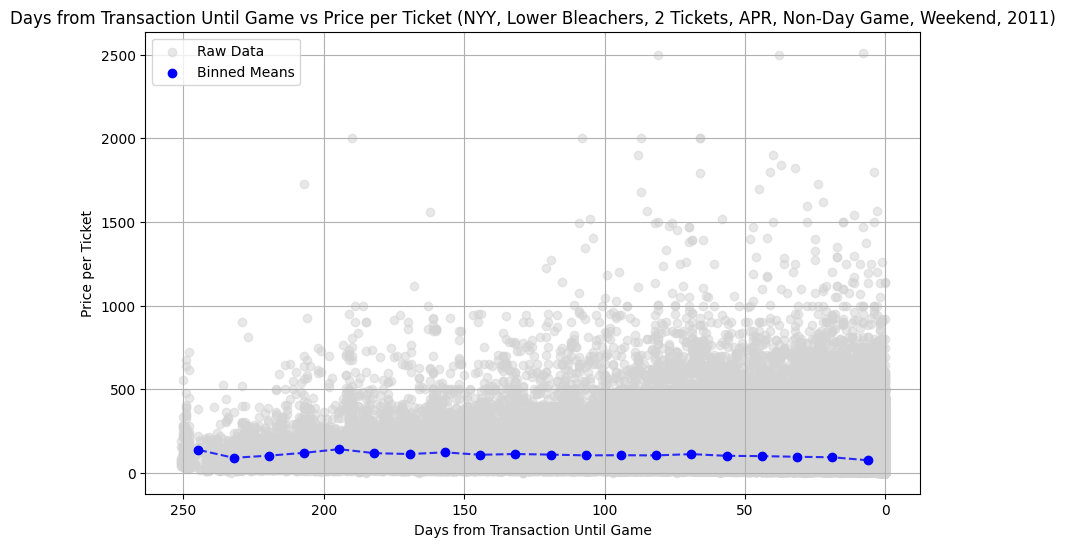
\includegraphics{images/10.png}

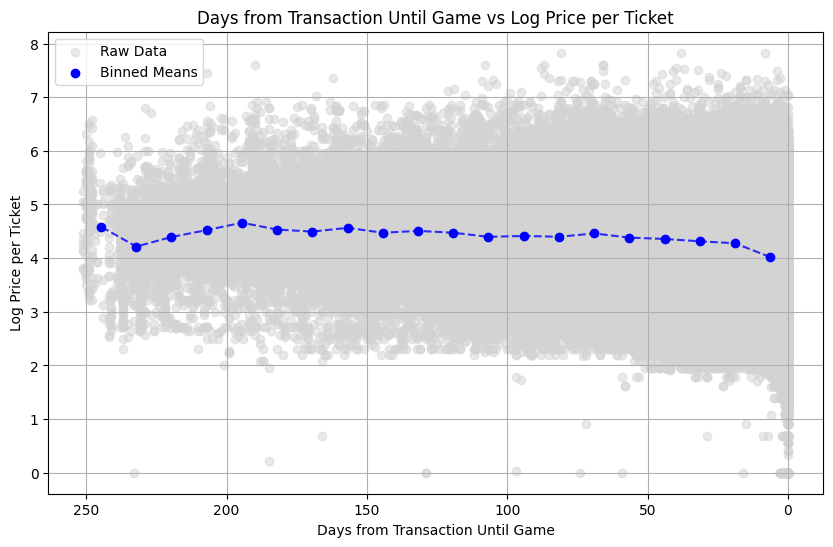
\includegraphics{images/8-01.png}

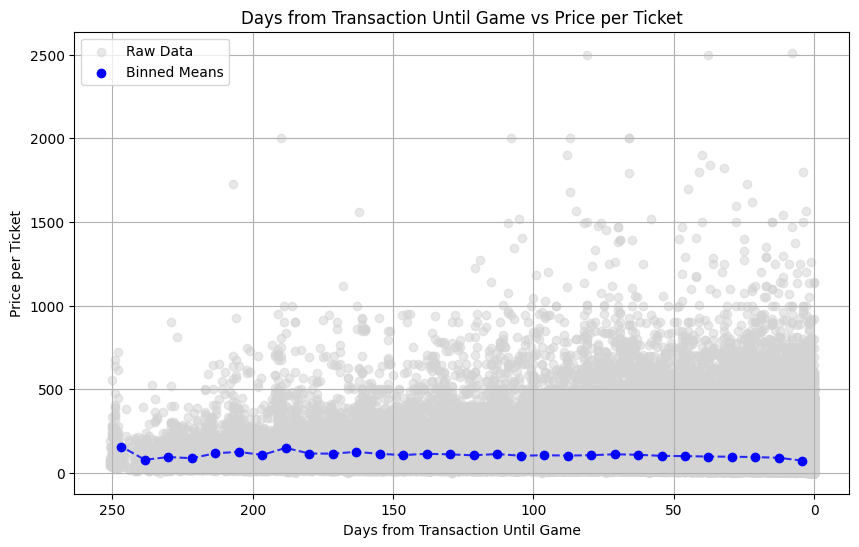
\includegraphics{images/7.png}

From this we see our regression results makes sense now. There are huge
outliers of people who pay more when game day is near (relative to when
game day is far). But on average people pay less when buying tickets
near game day. So to answer this question How do the prices consumers
pay for tickets change as the game date approaches (i.e., as the number
of days between transaction date and game date declines)? The initial
answer would be the prices \textbf{decrease} as game date approaches. To
further investigate the dynamic pattern, we would run a quasi ``event
study'' model to investigate. We show the distribution of transaction
and see there is bunching happening approximately every 8 days. There
are many reasons why this can be happening ranging from
discounts/promotions, timing of the games, etc. While we don't know why
exactly this is happening we can exploit these observations for our
event study model.

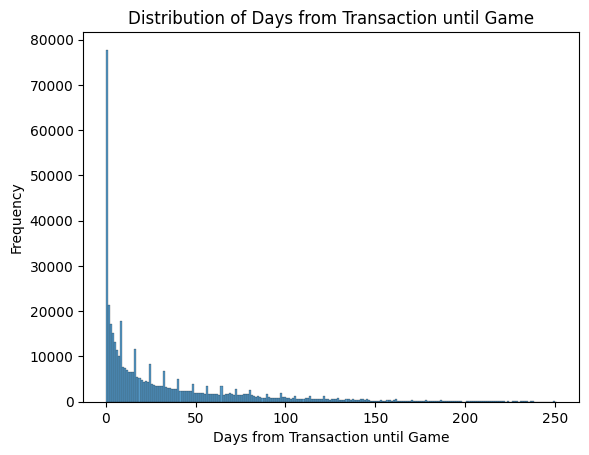
\includegraphics{images/6.png}

Using this observation we create our model.

\[
\text{price\_per\_ticket} = \beta_0 + \sum_{j=1}^{n} \beta_{1j} \cdot D_j \cdot \text{days\_until\_game} + \beta_2 \cdot \text{controls} + \beta_3 \cdot \text{num\_tickets} + \epsilon
\]

\subsection{Where:}\label{where}

\[
\mathbf{\mathrm{controls}} = \text{day\_game, weekend\_game, sectiontype, gamemonth, team, year}
\]

\begin{itemize}
\tightlist
\item
  \(\beta_0\) is the intercept.
\item
  \(\beta_{1j}\) is the coefficient for each range \(j\) of days from
  transaction until game:

  \begin{itemize}
  \tightlist
  \item
    \(D_1 = 1\) if days are in the range \(0-8\)
  \item
    \(D_2 = 1\) if days are in the range \(9-16\)
  \item
    \(D_3 = 1\) if days are in the range \(17-24\)
  \item
    \ldots{}
  \item
    \(D_n = 1\) for the last specified range (e.g., \(241-250\)).
  \end{itemize}
\item
  \(\beta_2 \cdot \mathbf{\text{controls}}\) represents a vector of
  control variables included in the model.
\item
  \(\beta_3\) is the coefficient for the number of tickets.
\item
  \(\epsilon\) is the error term.
\end{itemize}

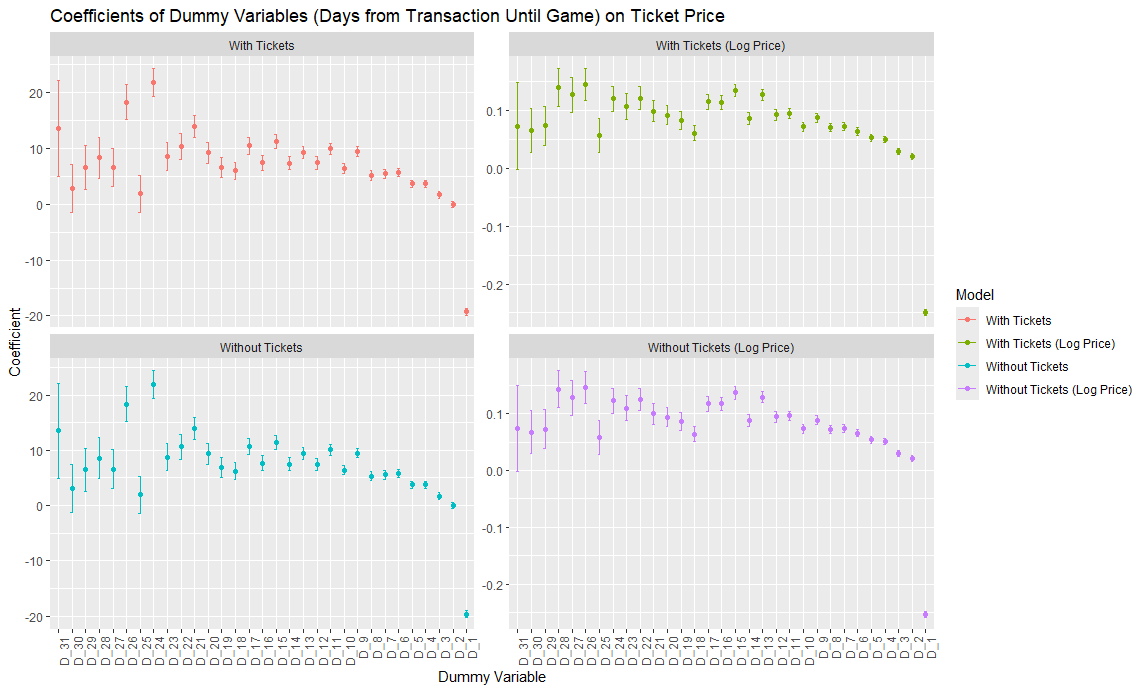
\includegraphics{images/12.png}

We see from this that the relationship may not be entirely linear. We
also see that ticket prices are in fact lower come one week before a
game, which supports previous results. One thing we did not take into
account for is the bias of human time perception. People typically think
of time between weeks, days and months, wherein overly long periods of
times are not referred to in weeks but in months. To study this, we run
the same model but take into account human biases, instead of cutting
the dummy variables in a 8 day basis, we cut up our dummy variables
based on human perceptions of months and weeks.

\[
\mathrm{price\_per\_ticket} = \beta_0 + \sum_{j=1}^{n} \beta_{1j} \cdot D_j \cdot \mathrm{days\_until\_game} + \beta_2 \cdot \mathrm{controls} + \beta_3 \cdot \mathrm{num\_tickets} + \epsilon
\]

\subsection{Where:}\label{where-1}

\[
\mathbf{\mathrm{controls}} = \mathrm{day\_game, weekend\_game, sectiontype, gamemonth, team, year}
\]

\begin{itemize}
\tightlist
\item
  \(\beta_0\) is the intercept.
\item
  \(\beta_{1j}\) is the coefficient for each range \(j\) of weeks and
  months from the transaction until the game:

  \begin{itemize}
  \tightlist
  \item
    \(D_1 = 1\) if the time until the game is in the range of 0-1 week
  \item
    \(D_2 = 1\) if the time until the game is in the range of 1-2 weeks
  \item
    \(D_3 = 1\) if the time until the game is in the range of 2-3 weeks
  \item
    \(D_4 = 1\) if the time until the game is in the range of 3-4 weeks
  \item
    \(D_5 = 1\) if the time until the game is in the range of 4-5 weeks
  \item
    \(D_6 = 1\) if the time until the game is in the range of 1-2 months
  \item
    \(D_7 = 1\) if the time until the game is in the range of 2-3 months
  \item
    \(D_8 = 1\) if the time until the game is in the range of 3-4 months
  \item
    \ldots{}
  \item
    \(D_n = 1\) if the time until the game is in the range of 8 to 8.3
    months, as the data concludes at 250 days.
  \end{itemize}
\item
  \(\beta_2 \cdot \mathbf{\text{controls}}\) represents a vector of
  control variables included in the model.
\item
  \(\beta_3\) is the coefficient for the number of tickets.
\item
  \(\epsilon\) is the error term.
\end{itemize}

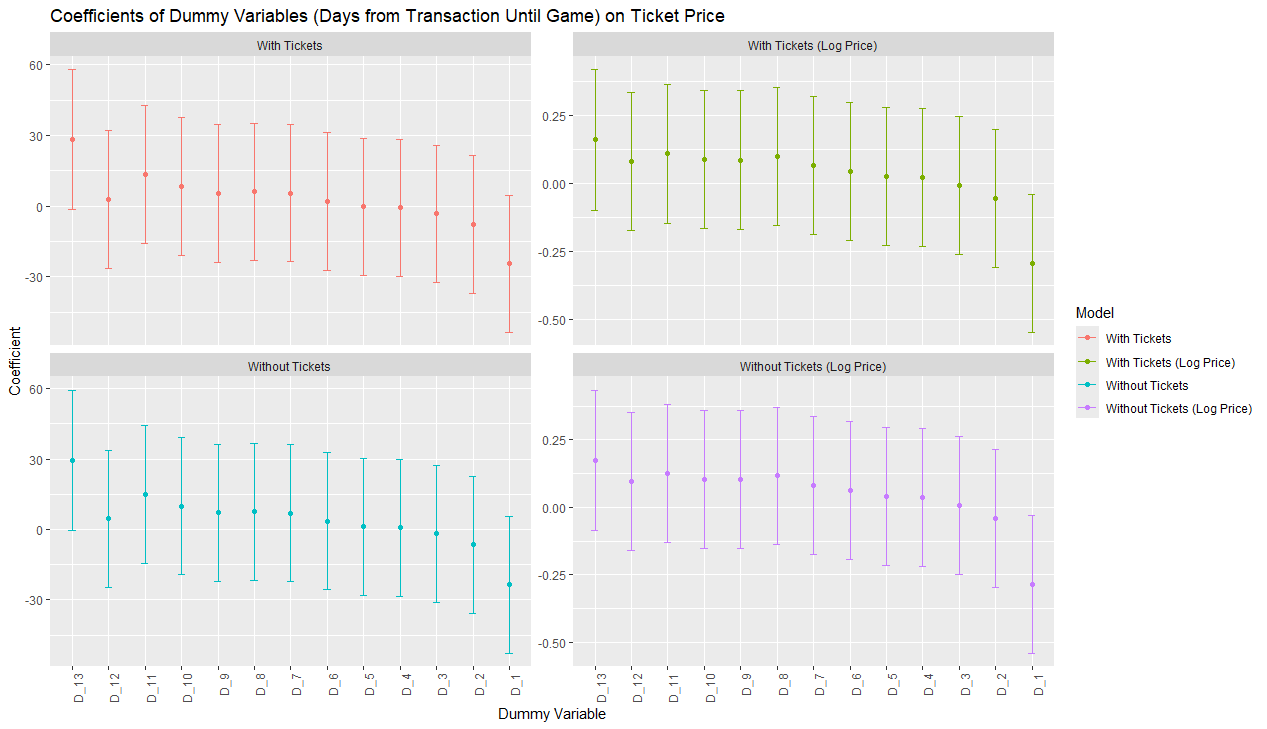
\includegraphics{images/13.png}

We see smoother and more observable relationship here. All this to
suggest that in fact, on average, the later you buy your tickets the
cheaper ticket prices would be. Next we study the year differences. We
look at the year coefficients of our main model.

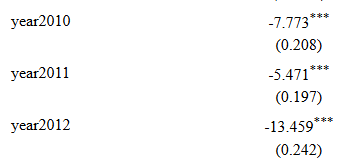
\includegraphics{images/14.png}

We see that there are significant year fixed effects that could be worth
investigating. Next, we run the same analysis restricting our
observations within each year.

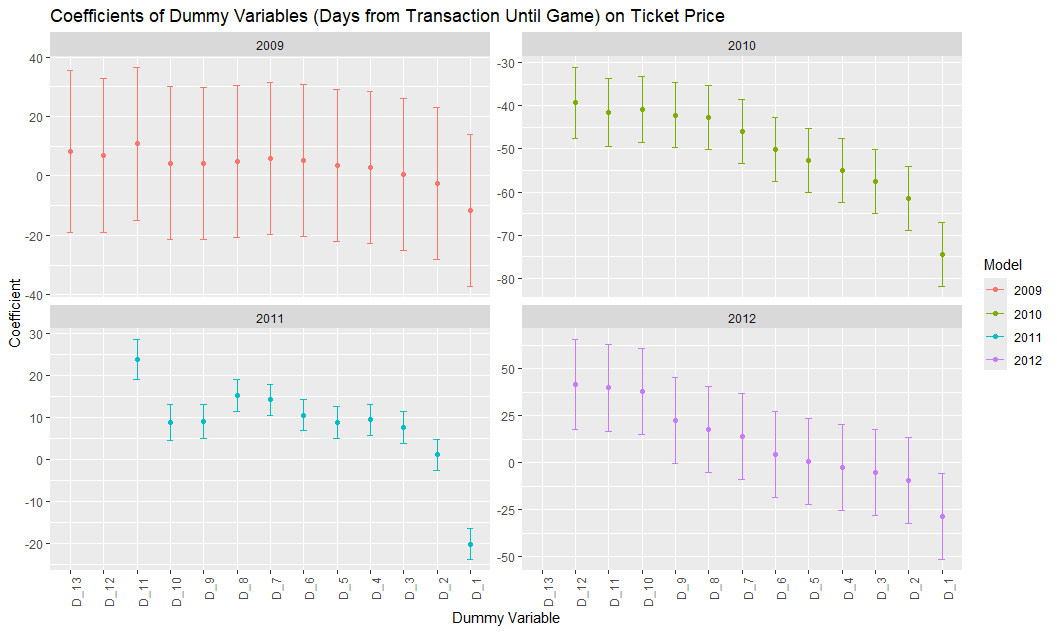
\includegraphics{images/15.png}

The observed trends reveal an interesting pattern: purchasing tickets
well in advance tends to result in higher ticket prices. However, there
are variations in this relationship over the years. For instance, in
2009, the standard error is notably large, indicating substantial
variability. During this year, some consumers were able to purchase
tickets far in advance (approximately 250 days before the game) at
prices comparable to those closer to game day.

In contrast, the dynamics shift in subsequent years, particularly in
2010, 2011, and 2012. The standard error becomes significantly smaller,
demonstrating greater consistency in pricing trends. As a result, a
clearer pattern emerges: tickets purchased closer to game day are
generally cheaper. By 2012, buying tickets just one week before the game
consistently results in lower prices, emphasizing the evolving dynamic
relationship between purchase timing and ticket cost.

\section{Task 2: Lottery Study}\label{task-2-lottery-study}

\subsection{Part I: Do any of the observations seem suspicious to
you?}\label{part-i-do-any-of-the-observations-seem-suspicious-to-you}

\subsubsection{1.Descriptive Data
Analysis}\label{descriptive-data-analysis}

The following are all my observations of the data. In summary,
\textbf{\texttt{Expend\_Total}} variable has a outlier with implausible
values, which has been removed. Duplicates are remoed as well. More
details are as follows.

\begin{itemize}
\item
  \textbf{Income and Age Variables:} The distributions of income and age
  appear normal based on the plots. These variables seem acceptable.
\item
  \textbf{Race}: The values for \texttt{black}, \texttt{hispanic}, and
  \texttt{white} align with the expected categories.
\item
  \textbf{Gender}: The data contains \texttt{male} and \texttt{female},
  but the manual specifies values should be:

  \begin{itemize}
  \item
    \texttt{1} for male
  \item
    \texttt{2} for female
  \item
    \texttt{3} for ``other.''\\
    This inconsistency needs to be addressed.
  \end{itemize}
\item
  \textbf{Marital Status}: The data includes values such as
  \texttt{married} and \texttt{0.0}, whereas the manual specifies:

  \begin{itemize}
  \item
    \texttt{1} for married
  \item
    \texttt{0} for not married.
  \end{itemize}
\item
  \textbf{Urban Residence}: The column contains \texttt{Metro\ Area} and
  \texttt{Non-Metro\ Area}, but it should be:

  \begin{itemize}
  \item
    \texttt{1} for urban (residing in a metropolitan area)
  \item
    \texttt{0} otherwise.
  \end{itemize}
\item
  \textbf{Employment and Religion Variables:} These variables seem
  acceptable.
\item
  \textbf{Years of Education:} This variable appears normal, and a plot
  has been attached for reference.
\item
  \textbf{Ideology:} The data contains values such as
  \texttt{Extremely\ Conservative}, \texttt{Moderate},
  \texttt{Slightly\ Conservative}, etc., but the manual specifies:

  \begin{itemize}
  \item
    \texttt{1} for extremely liberal
  \item
    \texttt{2} for liberal
  \item
    \texttt{3} for slightly liberal
  \item
    \texttt{4} for moderate
  \item
    \texttt{5} for slightly conservative
  \item
    \texttt{6} for conservative
  \item
    \texttt{7} for extremely conservative
  \end{itemize}
\item
  \textbf{State:} The data lists 51 states, which is incorrect as there
  are only 50 states in the U.S. This discrepancy needs investigation.
\item
  \textbf{Expend\_Total:} This variable is categorized as categorical in
  the data but should be numeric. Additionally, there are significant
  outliers, including an entry with a value of \texttt{100,000.0}. Some
  entries are not even numeric, requiring cleaning and conversion.
\item
  \textbf{Income\_Delta:} This variable appears normal, and a plot has
  been attached for verification.
\item
  \textbf{Expend\_Delta:} Although there are some outliers, the variable
  seems normal otherwise.
\item
  \textbf{Income\_Effects\_Delta\_Pct:} This variable is generally
  normal, apart from a few outliers.
\item
  \textbf{Risk-Seeking:} The data contains entries like \texttt{-3},
  \texttt{-4}, \texttt{-1\ -\ Very\ unwilling}, and
  \texttt{-7\ -\ Very\ willing}. However, the manual specifies the scale
  should range from \texttt{-7} to \texttt{-1}, where \texttt{-1} is
  ``very unwilling'' and \texttt{-7} is ``very willing.'' The
  inconsistent format needs correction.
\item
  \textbf{Risk Aversion:} This variable contains text entries, but it
  should include categorical numerical values:

  \begin{itemize}
  \item
    \texttt{1} for ``Substantial financial risks expecting to earn
    substantial returns''
  \item
    \texttt{2} for ``Above-average financial risks expecting to earn
    above-average returns''
  \item
    \texttt{3} for ``Average financial risks expecting to earn average
    returns''
  \item
    \texttt{4} for ``No financial risks.''
  \end{itemize}
\item
  \textbf{Seems\_Fun:} Entries include
  \texttt{-3\ -\ Strongly\ Disagree}, \texttt{0\ -\ Neutral}, and
  \texttt{3\ -\ Strongly\ Agree}, but the values should be on a scale
  from \texttt{-3} (strongly disagree) to \texttt{3} (strongly agree).
  The inconsistency requires recording.

  \begin{itemize}
  \tightlist
  \item
    Similar issues are present in \texttt{enjoy\_thinking} and
    \texttt{self\_control}.
  \end{itemize}
\item
  \textbf{Financial Literacy, Numeracy, and Related Columns:} Variables
  such as \texttt{financial\_literacy}, \texttt{financial\_numeracy},
  \texttt{non\_belief\_lln}, \texttt{ev\_miscalculation},
  \texttt{overconfidence}, and \texttt{lottery\_payout} appear normal.
\item
  \textbf{Happiness:} This column contains NaN values, which should be
  addressed during data cleaning.
\end{itemize}

\subsubsection{2. tabulation of income and
gender}\label{tabulation-of-income-and-gender}

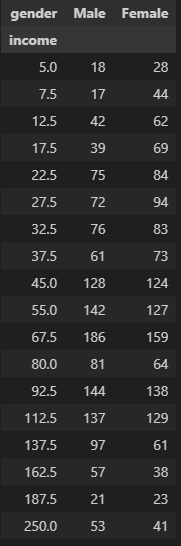
\includegraphics{images/4.png}

\subsubsection{3. Report detailed summary
statistics}\label{report-detailed-summary-statistics}

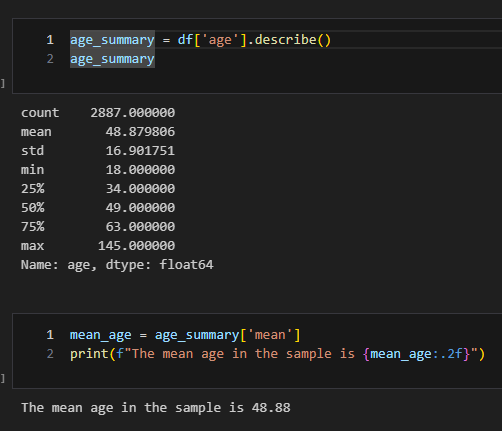
\includegraphics{images/9.png}

\subsubsection{4. Report summary
statistics}\label{report-summary-statistics}

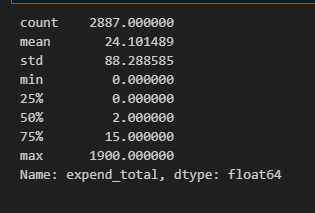
\includegraphics{images/10-03.png}

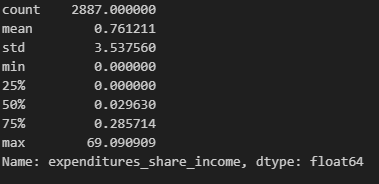
\includegraphics{images/11-03.png}

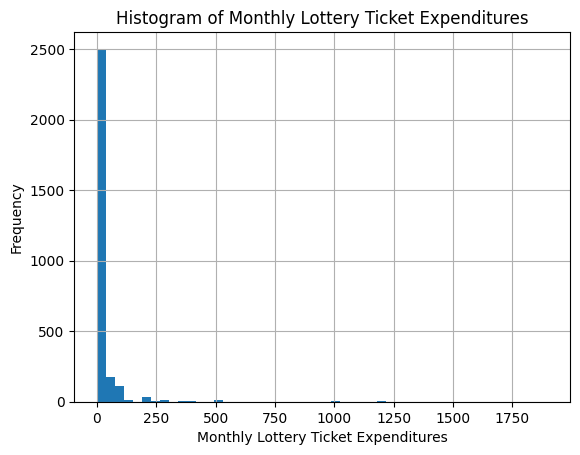
\includegraphics{images/12-02.png}

\subsubsection{5. Indicator Variable}\label{indicator-variable}

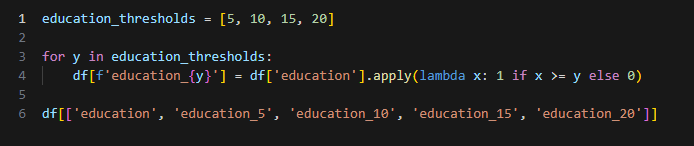
\includegraphics{images/13-01.png}

\subsubsection{6. How did changes in income from 2018 to 2019
vary}\label{how-did-changes-in-income-from-2018-to-2019-vary}

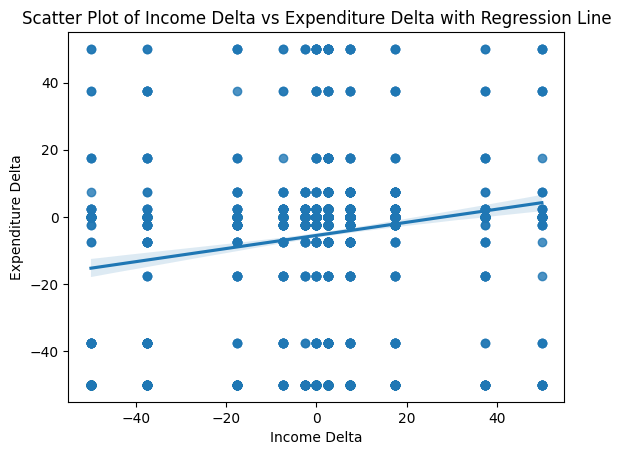
\includegraphics{images/16-01.png}

We see a positive relationship between income delta and expenditure
delta.

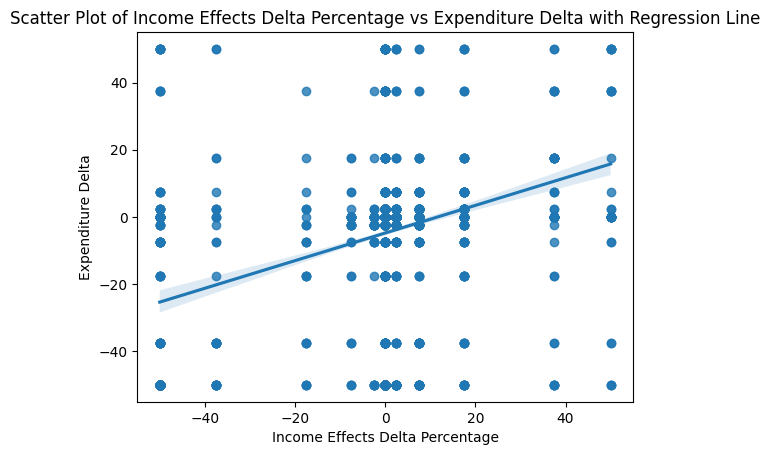
\includegraphics{images/17-01.png}

We see income effect delta and expenditure delta has a steeper positive
slope than income delta against expenditure delta. Overall, both plots
have similar variation.

\subsection{Part II Unpacking the determinants and correlates of lottery
expenditures}\label{part-ii-unpacking-the-determinants-and-correlates-of-lottery-expenditures}

\subsubsection{1.relationship between the monthly lottery expenditure
variable and
income.}\label{relationship-between-the-monthly-lottery-expenditure-variable-and-income.}

Below are my preliminary plots.

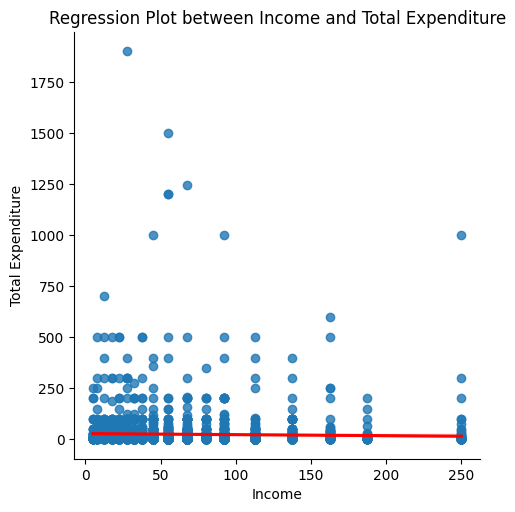
\includegraphics{images/18-01.png}

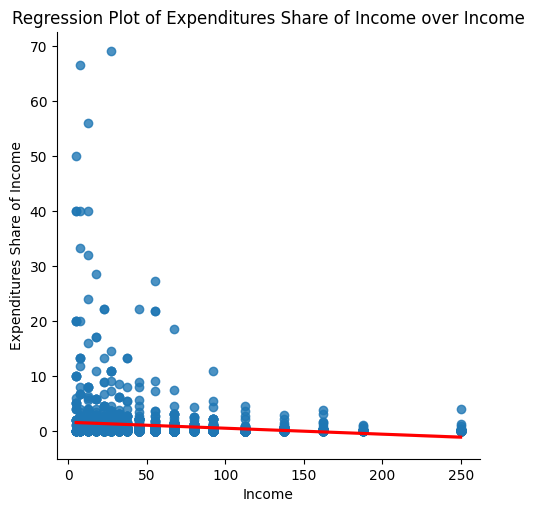
\includegraphics{images/19.png}

Previous knowledge on the topic suggests that higher-income individuals
tend to spend less on lotteries. However, based on our initial
observations, this does not appear to be the case. When plotting income
on the x-axis and lottery expenditure on the y-axis, we expect a
negative slope, reflecting the anticipated inverse relationship.
Instead, our observations reveal a nearly flat line, although there is a
slight downward trend.

Though, when examining lottery expenditure as a share of income, we find
that lower-income individuals allocate a larger proportion of their
income to lottery tickets compared to higher-income individuals. Some
observations show extreme cases where up to 70\% of income is spent on
lottery tickets, aligning with preconceived notions about lottery
spending behavior among low-income groups.

To investigate this further, we will conduct a multiple regression
analysis using cross-sectional data.

\begin{itemize}
\tightlist
\item
  \textbf{Dependent Variable}: Lottery expenditure\\
\item
  \textbf{Independent Variable}: Income\\
\item
  \textbf{Control Variables}: Age, race (Black, Hispanic, White),
  gender, marital status, urban residence, employment status, religion,
  education level, ideology, and state of residence.
\end{itemize}

To account for age-related life-cycle effects, we will create dummy
variables representing different age groups:\\
1. \textbf{Not Working Age}\\
2. \textbf{Early Working Age}\\
3. \textbf{Late Working Age}\\
4. \textbf{Retired}

These dummy variables will capture the differential effects across the
specified age categories. This approach provides a more nuanced
understanding of the relationships between income, demographic factors,
and lottery expenditure.

Additionally, I will use ideology as a continuous sliding scale ranging
from left (liberal) to right (conservative) as one of the variables in
the analysis.

The model is:

\[
Y_i = \beta_0 + \beta_1 \text{Income}_i + \sum_{j=1}^{p} \gamma_{j} C_{ij} + \sum_{k=1}^{q} \delta_k A_{ik} + \epsilon_i
\]

Where:\\
- \(Y_i\): Lottery expenditure (dependent variable)\\
- \(\text{Income}_i\): Individual income (main independent variable)\\
- \(\sum_{j=1}^{p} \gamma_j C_{ij}\): Summation over \(p\) control
variables (\(C_{ij}\)) with coefficients \(\gamma_j\). Control variables
include:

\begin{itemize}
\item
  Race (\(\text{Black}_i, \text{Hispanic}_i, \text{White}_i\)) - dummy
  variable
\item
  Gender - dummy variable
\item
  Marital status - dummy variable
\item
  Urban residence - dummy variable
\item
  Employment status - dummy variable
\item
  Religion - dummy variable
\item
  Education
\item
  Ideology
\item
  State - dummy variables
\item
  \(\sum_{k=1}^{q} \delta_k A_{ik}\): Summation over \(q\) age
  life-cycle dummies (\(A_{ik}\)) with coefficients \(\delta_k\). These
  variables are:

  \begin{itemize}
  \item
    \textbf{NotWorkingAge}: \(A_{i1} = 1\) if age \(< 15\), else
    \(A_{i1} = 0\)
  \item
    \textbf{EarlyWorkingAge}: \(A_{i2} = 1\) if
    \(15 \leq \text{age}_i < 30\), else \(A_{i2} = 0\)
  \item
    \textbf{LateWorkingAge}: \(A_{i3} = 1\) if
    \(30 \leq \text{age}_i < 60\), else \(A_{i3} = 0\)
  \item
    \textbf{Retired}: \(A_{i4} = 1\) if \(\text{age}_i \geq 60\), else
    \(A_{i4} = 0\)
  \end{itemize}
\item
  \(\epsilon_i\): Error term
\end{itemize}

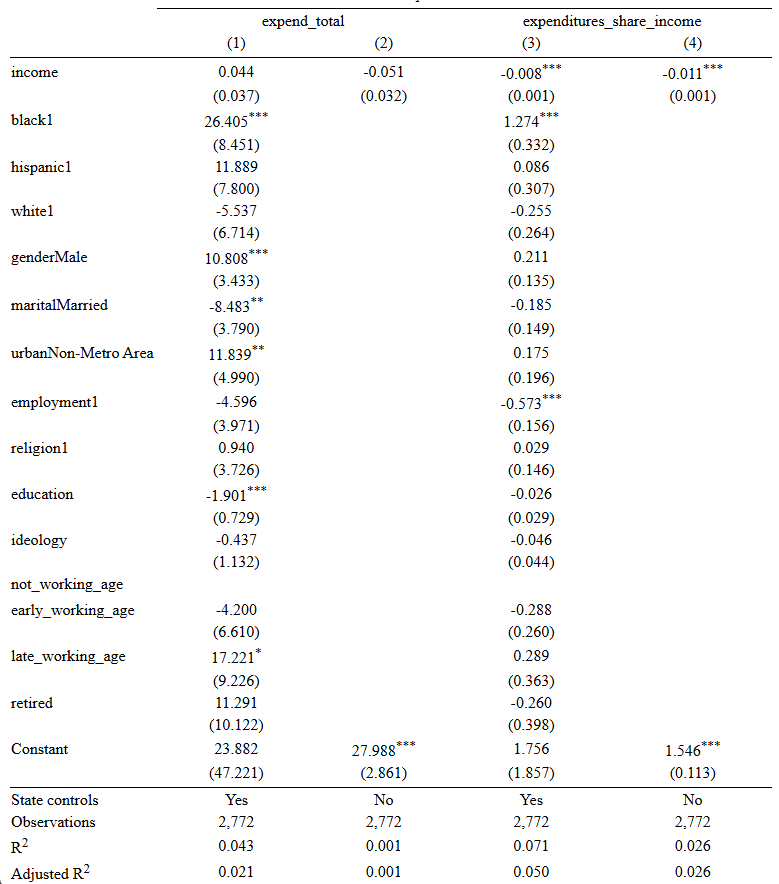
\includegraphics{images/5-01.png}

Our findings indicate that \textbf{the relationship between income and
lottery ticket expenditure is weak.} After controlling for variables
such as race, gender, marital status, urban location, employment,
religion, education, ideology, and age, we identified that more
significant determinants of lottery expenditure include education,
working age, race, gender, marital status, urban area, and age life
cycle. When we use expenditure as a share of income as our dependent
variable, the results align with our previous observations from the
scatter plot. Specifically, \textbf{individuals with higher incomes tend
to spend a smaller proportion of their income on lottery tickets}. This
effect remains consistent even with all the controls mentioned earlier.
Additionally, the results suggest that employment and race are more
significant variables when it comes to ticket expenditure as a share of
income.

\subsubsection{2. Monthly lottery expenditure variable and bias proxy
variables}\label{monthly-lottery-expenditure-variable-and-bias-proxy-variables}

I will explore the relationship between the monthly lottery expenditure
variable and the preference and bias proxy variables. To achieve this, I
will utilize the following variables: risk\_seeking, risk\_aversion,
seems\_fun, enjoy\_thinking, overconfidence, and happiness. I plan to
employ Principal Component Analysis (PCA) to combine these variables
into a single composite variable that captures an individual's overall
likelihood of being interested in participating in a lottery ticket.

Next, I will incorporate a self\_control variable to represent an
individual's impulse control, distinguishing it from their interest in
participating in a lottery.

Lastly, I will again use PCA to create a composite variable from the
following state variables: financial\_literacy, financial\_numeracy,
gamblers\_fallacy, non\_belief\_lln, and ev\_miscalculation. This
composite variable will capture an individual's understanding of risk
and reward when participating in a lottery ticket.

Through this analysis, I aim to identify specific biases that influence
lottery participation and determine which aspects of bias play a more
significant role in this behavior.

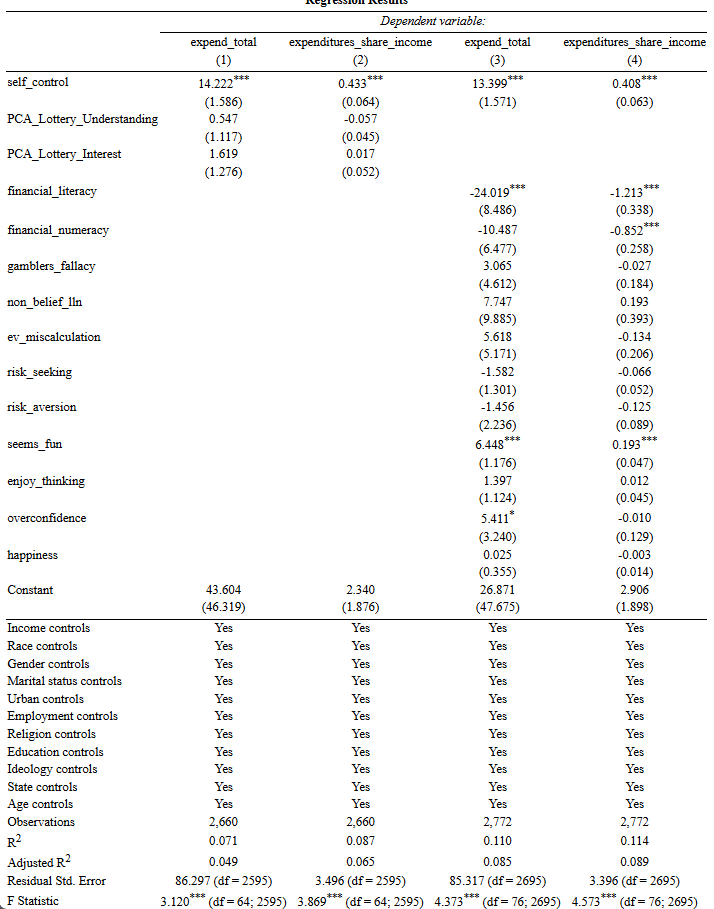
\includegraphics{images/6-01.png}

Examining our PCA variables, we find that the measures for lottery
understanding and lottery interest are insignificant. This suggests that
lottery understanding and interest do not significantly influence
lottery expenditure. On the other hand, self-control is significant,
indicating that the aspect of self-control plays a critical role in
driving lottery activity, potentially due to addictive behaviors.

These findings suggest that behavioral biases, particularly those
related to self-control, play a substantial role in lottery
expenditures. This may point to a form of addiction underlying lottery
behavior.

To further study our created PCA variables, I analyze the correlation
matrices underlying our PCA variables and compare them to our known
controls and fixed effects.

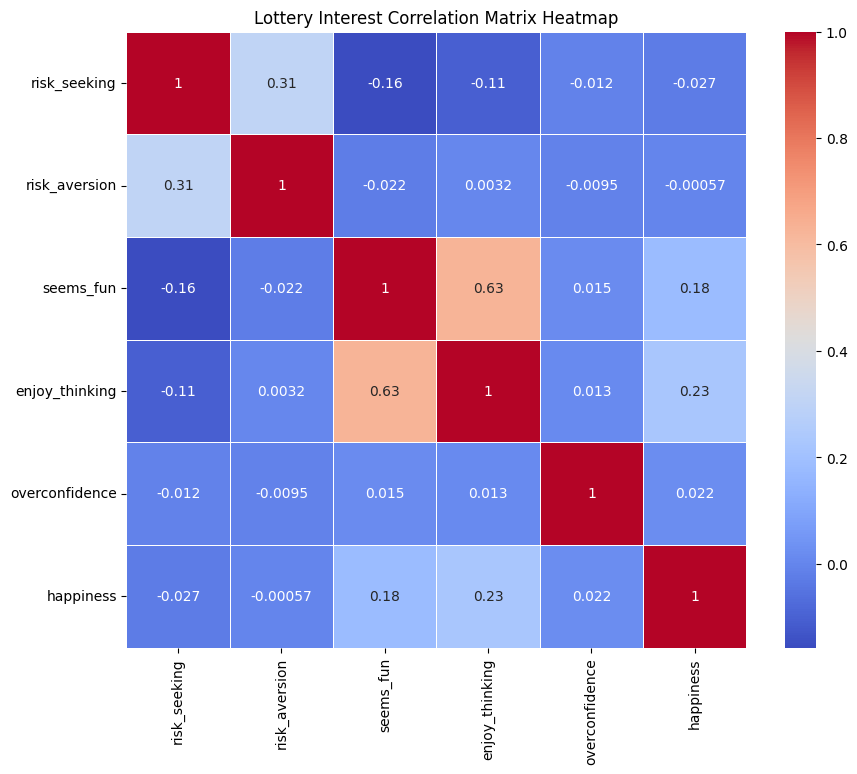
\includegraphics{images/20.png}

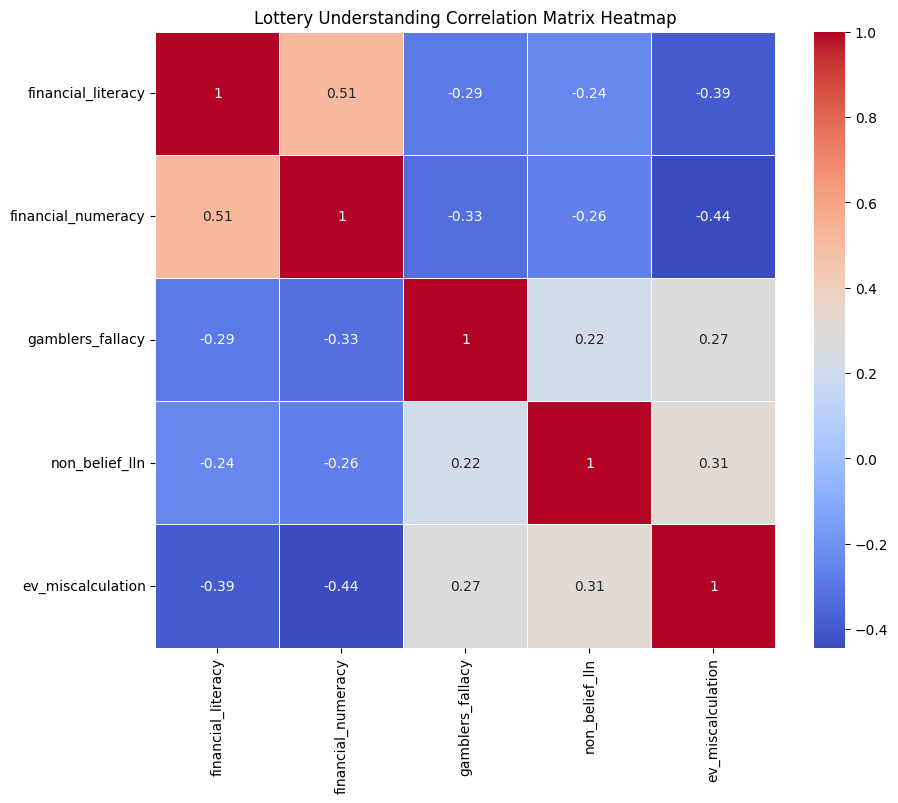
\includegraphics{images/21.png}

We see that majority of the variables are uncorrelated. This could be a
reason why our PCA variables are insignificant. With this observation in
mind, I decompose my PCA variables into their underlying variables and
run the regression with the underlying variables. The result are as
follows.

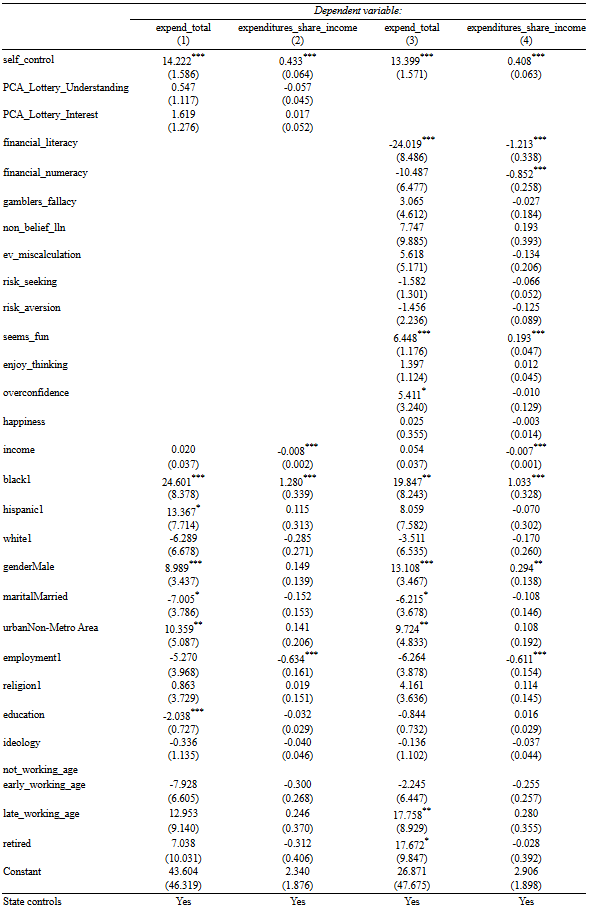
\includegraphics{images/7-01.png}

This analysis reveals that some behavioral biases significantly
influence lottery expenditures. The coefficients for self-control and
financial literacy are comparable, if not greater, than those of
previously mentioned significant variables for lottery expenditure, such
as race (being Black), gender (being male), and being in the late
working age group. Overall, the data suggest that while some behavioral
biases do impact lottery expenditure, only very specific biases are
significant; most behavioral biases do not have a meaningful effect on
lottery expenditures.

\subsection{PART III -- Short Answer}\label{part-iii-short-answer}

\subsubsection{A. Share of the total prize pool added to sub-pool by
Mega
Millions}\label{a.-share-of-the-total-prize-pool-added-to-sub-pool-by-mega-millions}

Please see this
\href{https://files.floridalottery.com/exptkt/megaMillions-GameRules.pdf}{link},
outlining Florida's mega millions lottery for 2020
\citep{lotteryMEGAMILLIONSGame2020}

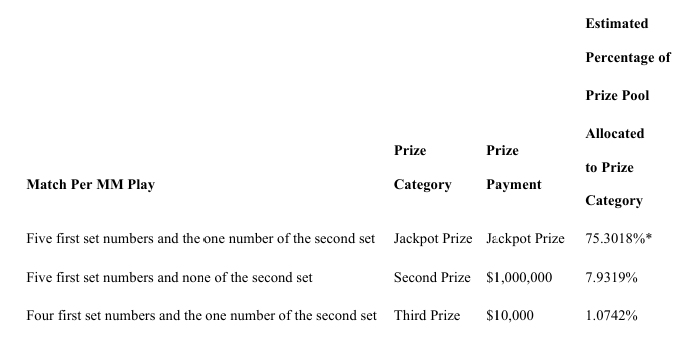
\includegraphics{images/8.png}

\subsubsection{B Interesting economics paper that you have recently
read}\label{b-interesting-economics-paper-that-you-have-recently-read}

An interesting paper I recently came across is \emph{Worth Your Weight:
Experimental Evidence on the Benefits of Obesity in Low-Income
Countries} by Elisa Macchi (2023), published in the \emph{American
Economic Review} \citep{macchiWorthYourWeight2023}. I found this
particularly fascinating because it quantifies the economic benefits of
obesity in credit markets within developing countries.

Coming from a developing country, I've often heard anecdotally about the
association between obesity and wealth or prosperity. However, in more
developed countries, obesity is frequently linked to poverty. Living in
a developed country, this created a striking contrast in my mind, on the
economic structures that lead to this observation.

What stood out to me in this paper was the use of face morphing
technology, which I believe represents a relatively new and unique tool
in economic research. The study demonstrated that obesity acts as a
beneficial signal only in markets where other indicators of wealth or
creditworthiness are absent. In such environments, obesity or luxury
goods serve as signals to facilitate credit access.

This led me to reflect on the role of wealth signals in both developing
and developed countries. Why do these signals work effectively in some
settings but not in others? Wouldn't similar mechanisms apply in
developed countries as well? If not, why are obesity and luxury goods
less prevalent as signals in developed countries compared to developing
ones? Is the difference primarily cultural or institutional? I would be
very interested in seeing a similar study conducted in developed
countries to determine whether these results align across contexts.


  \bibliography{bibliography.bib}


\end{document}
